\documentclass[a4paper,12pt]{amsart}

\usetheme[progressbar=frametitle]{metropolis}
\metroset{block=fill}

\subtitle{NTIN071 Automata and Grammars}
\author{Jakub Bulín (KTIML MFF UK)}

\date{Spring 2025\\ 
    \vspace{1in} 
    \begin{flushleft}
        \it \footnotesize * Adapted from the Czech-lecture slides by Marta Vomlelová with gratitude. The translation, some modifications, and all errors are mine.
    \end{flushleft}
}

%% packages

\usepackage{amsmath}
\usepackage{amssymb}
\usepackage{amsthm}
\usepackage{cancel}
\usepackage{color}
\usepackage{colortbl}
\usepackage{forest}
\usepackage[utf8x]{inputenc}
\usepackage{multicol}
\usepackage{multirow}

%% colors
\definecolor{Gray}{gray}{0.9}

%% TikZ
\usepackage{tikz}
    \usetikzlibrary{
        automata,
        arrows,
        backgrounds,
        decorations.pathmorphing,
        fit,
        positioning,
        shapes,
        shapes.geometric,
        tikzmark
    } 
    \tikzset{>=stealth',shorten >=1pt,auto,node distance=2cm}
    \tikzset{initial text={}}
    \tikzset{elliptic state/.style={draw,ellipse}}

%% amsthm
\theoremstyle{plain}
    \newtheorem*{algorithm}{Algorithm}    
    \newtheorem*{observation}{Observation}
    \newtheorem*{proposition}{Proposition}

\theoremstyle{remark}
    \newtheorem*{exercise}{Exercise}
    \newtheorem*{remark}{Remark}

%% macros
\DeclareMathOperator{\RegE}{RegE}
\DeclareMathOperator{\RL}{RL}

% Just for Lecture 2
\newcommand{\x}{$\times$}
\newcommand{\nx}{\ }


\begin{document}

\thispagestyle{empty}

\section*{NTIN071 A\&G: Tutorial 7 -- Chomsky normal form, The CYK algorithm}

\medskip

\subsection*{Teaching goals:} The student is able to

    \begin{itemize}\setlength{\itemsep}{0pt}
        \item 
    \end{itemize}


\section*{In-class problems}


\medskip\begin{problem}

\end{problem}


\section*{Extra Practice and Thinking}


\medskip\begin{problem}

\end{problem}


\end{document}



\documentclass[a4paper,12pt]{amsart}

\usetheme[progressbar=frametitle]{metropolis}
\metroset{block=fill}

\subtitle{NTIN071 Automata and Grammars}
\author{Jakub Bulín (KTIML MFF UK)}

\date{Spring 2025\\ 
    \vspace{1in} 
    \begin{flushleft}
        \it \footnotesize * Adapted from the Czech-lecture slides by Marta Vomlelová with gratitude. The translation, some modifications, and all errors are mine.
    \end{flushleft}
}

%% packages

\usepackage{amsmath}
\usepackage{amssymb}
\usepackage{amsthm}
\usepackage{cancel}
\usepackage{color}
\usepackage{colortbl}
\usepackage{forest}
\usepackage[utf8x]{inputenc}
\usepackage{multicol}
\usepackage{multirow}

%% colors
\definecolor{Gray}{gray}{0.9}

%% TikZ
\usepackage{tikz}
    \usetikzlibrary{
        automata,
        arrows,
        backgrounds,
        decorations.pathmorphing,
        fit,
        positioning,
        shapes,
        shapes.geometric,
        tikzmark
    } 
    \tikzset{>=stealth',shorten >=1pt,auto,node distance=2cm}
    \tikzset{initial text={}}
    \tikzset{elliptic state/.style={draw,ellipse}}

%% amsthm
\theoremstyle{plain}
    \newtheorem*{algorithm}{Algorithm}    
    \newtheorem*{observation}{Observation}
    \newtheorem*{proposition}{Proposition}

\theoremstyle{remark}
    \newtheorem*{exercise}{Exercise}
    \newtheorem*{remark}{Remark}

%% macros
\DeclareMathOperator{\RegE}{RegE}
\DeclareMathOperator{\RL}{RL}

% Just for Lecture 2
\newcommand{\x}{$\times$}
\newcommand{\nx}{\ }


\begin{document}

% \thispagestyle{empty}

\section*{NTIN071 A\&G: Tutorial 7 -- Formal grammars, regular and context-free grammars, bonus: two-way automata}

% second tutorial after Lecture 6
% spring 2024

\medskip

\noindent\emph{Solve 1a-d, 2, 3, 4ab first (the rest is for practice, the bonus section on 2-way automata won't be tested)}

\medskip


\medskip\begin{problem}[Constructing grammars]

    Design grammars (of the highest possible type) which generate the following languages (the alphabet is $\Sigma=\{a,b\}$ unless specified otherwise).
    
    \begin{multicols}{2}
    \begin{enumerate}[(a)]    
        \item $L=\Sigma^*$
        \item $L=\{w\mid |w|_b\text{ is even}\} $
        \item $L=\{ww^R\mid w\in \Sigma^*\} $
        \item $L=\{a^{2i}b^j\mid i\leq j\}$
        \item $L=\{w\mid |w|_a = 2|w|_b\}$
        \item $L = \{a^ib^jc^k\mid i = j\text{ or }j = k\}$    
    \end{enumerate}
    \end{multicols}

\end{problem}


\medskip\begin{problem}[FA to grammar]

    For the following automaton, find an equivalent grammar. Which class of the Chomsky hierarchy does it belong to?
    
    \begin{center}
        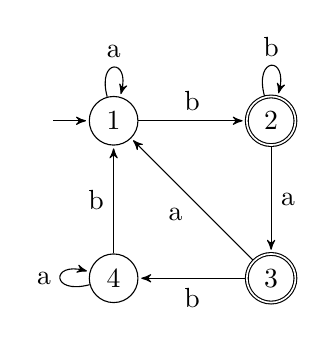
\begin{tikzpicture}[>=stealth',shorten >=1pt,auto,node distance=2cm]
            \tikzset{every state/.style={minimum size=0.2cm}}			
            \node[initial,state]  (a1)      {1};
            \node[state,accepting] (b1)  [right of=a1]    {2};
            \node[state,accepting] [below of=b1](c1)      {3};
            \node[state] [below of=a1](d1)      {4};
            \path[->]
                (a1)  edge  node {b} (b1)
                (a1)  edge[loop above]  node {a} (a1)
                (b1)  edge[loop above]  node {b} (b1)
                (d1)  edge[loop left]  node {a} (d1)
                (b1)  edge  node {a} (c1)
                (c1)  edge  node {a} (a1)
                (c1)  edge  node {b} (d1)
                (d1)  edge  node {b} (a1);
        \end{tikzpicture}
    \end{center}
        
\end{problem}


\medskip\begin{problem}[Type 3 grammar to FA] 
    
    For the following right linear grammar, construct an equivalent finite automaton: $G=(\{S,A,B,C\},\{a,b\},\mathcal P,S)$ where $\mathcal P$ consists of the following production rules:

    \bigskip
        
    \begin{center}
        \begin{tabular}{l}
            $S\rightarrow abS\mid babA\mid \epsilon $\\
            $A\rightarrow abA\mid aB \mid  bC$\\
            $B\rightarrow abS\mid B\mid bC\mid \epsilon $\\
            $C\rightarrow aab\mid A\mid aA\mid \epsilon $
        \end{tabular}
    \end{center}
    
\end{problem}


\medskip\begin{problem}[Testing properties of context-free languages]
    
    Design an (efficient) algorithm which decides in a given CFG satisfies the given property:
    
    \medskip

    \begin{enumerate}[(a)]
        \item $L(G)\neq\emptyset$
        \item $\epsilon\in L(G)$
        \item $L(G)$ is a finite language
    \end{enumerate}

\end{problem}
    

\medskip\begin{problem}[Small grammars generating large (finite) languages]
    
    Find a sequence of CFGs $G_1,G_2,G_3,\dots$ (over a given alphabet $\Sigma$) such that $G_n$ generates exactly all words of length $\leq 2^n$ (and no other words), and the size of $G_n$ (for simplicity, say the number of symbols in bodies of production rules) is in $O(n)$.
    
    %X_1 \to X_2_X2, X_2 \to X_3X_3,\dots, X_{n−1}\to X_nX_n, X_n\to aa|a|\epsilon

\end{problem}


\bigskip

\end{document}